% !TeX spellcheck = es_ES
\documentclass[titlepage,11pt]{article}
\usepackage[spanish,mexico]{babel}
% !TeX root = informe.tex
\usepackage{alphalph}
\makeatletter
\newcommand*{\fnsymbolsingle}[1]{%
	\ensuremath{%
		\ifcase#1%
		\or *%
		\or \dagger
		\or \ddagger
		\or \mathsection
		\or \mathparagraph
 		\or	\diamond
 		\or	\aleph
% 		\or	\backepsilon %needs amssymb or something
 		\or	\flat
		\else
		\@ctrerr
		\fi
	}%
}
 \newcommand*{\myfnsymbol}[1]{%
 	\myfnsymbolsingle{\value{#1}}%
 }

\makeatother
\newalphalph{\fnsymbolmult}[mult]{\fnsymbolsingle}{}
\renewcommand*{\thefootnote}{%
\fnsymbolmult{\value{footnote}}%
}









%\usepackage{alphalph}
%\makeatletter
% \newcommand*{\myfnsymbolsingle}[1]{%
% 	\ensuremath{%
% 		\ifcase#1% 0
% 		\or % 1
% 		*%   
% 		\or % 2
% 		\dagger
% 		\or % 3  
% 		\ddagger
% 		\or % 4   
% 		\mathsection
% 		\or % 5
% 		\mathparagraph
% 		\or
% 		\diamond
% 		\or
% 		\aleph
% 		\or
% 		\backepsilon
% 		\or
% 		\flat
% 		\else % >= 7
% 		\@ctrerr  
% 		\fi
% 	}%   
% }   
% \makeatother
% 
% \newcommand*{\myfnsymbol}[1]{%
% 	\myfnsymbolsingle{\value{#1}}%
% }
%%  remove upper boundary by multiplying the symbols if needed
%
% \newalphalph{\myfnsymbolmult}[mult]{\myfnsymbolsingle}{}
% \renewcommand*{\thefootnote}{%
% 	\myfnsymbolmult{\value{footnote}}%
% }
\usepackage{graphicx, tikz, subcaption}

\usepackage[onehalfspacing]{setspace}


% HYPERREF
\usepackage{xcolor}
%\definecolor{visigrey}{rgb}{.1,.15,.15}
\definecolor{darkblue}{rgb}{0,0,.6}
\usepackage[
	allcolors=darkblue,%visigrey,
	colorlinks=true,
]{hyperref} %Hyperref antes de geometry!

\usepackage{pdfpages}
\usepackage[a4paper,left=2cm,right=2cm]{geometry}
\geometry{top=1cm,bottom=.5cm}
\savegeometry{titlepage}
\geometry{top=2cm,bottom=2cm}
\savegeometry{main}
\usepackage{pgfplots,tikz,graphicx}
\usepackage{filecontents}
\def\bspace{\(\qquad\qquad\qquad\)}
\usepackage[T1]{fontenc}
\usepackage[utf8]{inputenc}
%\usepackage{sansmathfonts}
\usepackage{lmodern}
%\renewcommand*\familydefault{\sfdefault}
\usepackage[square,numbers,sort]{natbib} % sort=en orden de aparición
\bibliographystyle{unsrtnat}

\setcounter{tocdepth}{2}
% FOOTNOTE
\usepackage{todonotes}
\usepackage{pdfpages}


\def\changemargin#1#2{\list{}{\rightmargin#2\leftmargin#1}\item[]}
\let\endchangemargin=\endlist 
\pgfplotsset{compat=1.16}






\usepackage{listings}
\usepackage{xcolor}

%New colors defined below
\definecolor{codegreen}{rgb}{0,0.6,0}
\definecolor{codegray}{rgb}{0.5,0.5,0.5}
\definecolor{codepurple}{rgb}{0.58,0,0.82}
\definecolor{backcolour}{rgb}{0.95,0.95,0.92}

%Code listing style named "mystyle"
\lstdefinestyle{mystyle}{
  backgroundcolor=\color{backcolour},   commentstyle=\color{codegreen},
  keywordstyle=\color{magenta},
  numberstyle=\tiny\color{codegray},
  stringstyle=\color{codepurple},
  basicstyle=\ttfamily\footnotesize,
  breakatwhitespace=false,         
  breaklines=true,                 
  captionpos=b,                    
  keepspaces=true,                 
  numbers=left,                    
  numbersep=5pt,                  
  showspaces=false,                
  showstringspaces=false,
  showtabs=false,                  
  tabsize=2
}

\lstset{style=mystyle} 
\usepackage[scaled=0.85]{FiraMono}
\usepackage{listings}
\usepackage{hyperref}

\lstset{basicstyle = \ttfamily,
        keywordstyle=\bfseries,
        language = Python,
        tabsize=4,
        escapeinside={`}{`}
        }

%\usepackage{bigfoot} % to allow verbatim in footnote
%
% \let\ph\mlplaceholder % shorter macro
% \lstMakeShortInline"

% \renewcommand{\lstlistingname}{Código}
% \renewcommand{\lstlistlistingname }{Códigos \Matlab}
% \lstset{
%   language           =  Python
%   basicstyle         = \mlttfamily,
%   escapechar         = ",
%   mlshowsectionrules = true,
%   numbers = none,
%   tabsize=4,
% }
 % Mostrar codigo python
% GLOSARIO
\usepackage[sort=none,abbreviations]{glossaries-extra}
\setabbreviationstyle{long-short}

% \newabbreviation{fem}
% {FEM}
% {modelo de elementos finitos}


\newglossaryentry{quantumeff}
{
	name=Quantum Efficiency,
	text=quantum efficiency,
	description={Razón de conversión de fotón a electrón para un sensor. Depende de la longitud de onda.}
}

% \newglossaryentry{lst}
% {
% 	name=Linear Strain Triangle,
% 	text=LST,
% 	description={Elemento triangular de 6 nodos. Puede captar gradientes lineales de tensión con precisión arbitraria.}
% }
 
%% DIFFERENTIAL OPERATOR
\makeatletter
\providecommand*{\diff}%
{\@ifnextchar^{\DIfF}{\DIfF^{}}}
\def\DIfF^#1{%
	\mathop{\mathrm{\mathstrut d}}%
	\nolimits^{#1}\gobblespace}
\def\gobblespace{%
	\futurelet\diffarg\opspace}
\def\opspace{%
	\let\DiffSpace\!%
	\ifx\diffarg(%
	\let\DiffSpace\relax
	\else
	\ifx\diffarg[%
	\let\DiffSpace\relax
	\else
	\ifx\diffarg\{%
	\let\DiffSpace\relax
	\fi\fi\fi\DiffSpace}
	

\def\Matlab{\(\textrm{\textsc{Matlab}}\)}%^\textrm{®}

\def\metano{\ensuremath{\mathrm{CH}_4}}
\newcommand{\oxygen}{\ensuremath{\textrm{O}_2}}
\newcommand{\dioxcarb}{\ensuremath{\textrm{CO}_2}}
\newcommand{\dioxsulf}{\ensuremath{\textrm{SO}_2}}
\renewcommand{\d}[1]{\ensuremath{\operatorname{d}\!{#1}}}
\newcommand{\sat}{{\tiny\textrm{sat}}}
\newcommand{\SOx}{\ensuremath{\textrm{SO}_x}}
\newcommand{\NOx}{\ensuremath{\textrm{NO}_x}}

\def\micro{\ensuremath{\mu}}
\def\px{\ensuremath{\mathrm{px}}}
\def\pixrad{\ensuremath{I_{\px}}}
\def\radiance{\ensuremath{I_R}}
\def\radianceunits{\ensuremath{\text{W}\,\text{m}^{-2}\,\text{sr}^{-1}}}
\def\pixradunits{\ensuremath{\text{W}\,\text{m}^{-2}\,\text{sr}^{-1}\,\micro \text{m}^{-1} }}

\def\LEO{\ensuremath{{\mathrm{\tiny LEO}}}}
\def\earth{\ensuremath{\mathrm{tierra}}}
\def\sensor{\ensuremath{{\! \mathrm{\footnotesize sens}}}}



\def\simulationGraphic{
\begin{figure}[htb!]
\centering
\pgfplotsset{colormap/jet}
	\begin{tikzpicture}	
		\begin{axis}[view={30}{40}, width=0.7\textwidth,y dir=reverse,
		title={Radiancia de píxel a 100km de altura},xlabel={Longitud de onda [\micro m]},
		ylabel={Concentración de \metano [ppm]}, zlabel={\pixrad~  [\pixradunits]}]
		\addplot3 [surf, mesh/rows=7, shader=faceted interp]
		table[x=wl, y=ch, z=ir, col sep=comma] {plots/ch4ppmSurf-M7.csv};
		\addplot3 [mesh, black, mesh/rows=7, shader=faceted interp]		table[x=wl, y=ch, z=ir, col sep=comma] {plots/ch4ppmSurf-M7.csv};
		\end{axis}
	\end{tikzpicture}
	\caption{Grafico  de radiancia de píxel en función de longitud de onda y concentración de \metano.}
	\label{fig:ch4IrrVsPpm}
\end{figure}
} % macros para matematica en su mayor parte


\usepackage{float}
%% CARATULA
\def\autor{SpaceMeters \and Pato}
\def\carrera{Open Space}
\def\empresa{}

\def\tema{Informe de avance}
\def\titulo{Mapeo de gases contaminantes en la atmósfera por medio de instrumentos de medición de bajo costo}


\def\fecha{\today}
\def\colorborde{white} % black or 'white' para que no tenga borde



\begin{document}

\def\headingtype{\bf \small}
\def\openspacelogo{\href{https://www.spaceisopen.com/}{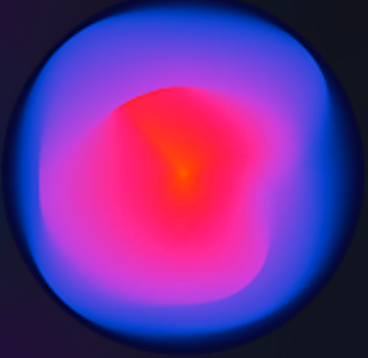
\includegraphics[height=25mm, clip]{caratula/logo}}}

\loadgeometry{titlepage}
\begin{titlepage}
	\centering
	\begin{tikzpicture}[remember picture, overlay]
	\coordinate (top_right) at 
	([xshift=-2.5cm, yshift=-2.5cm]current page.north east);
	\coordinate (top_left) at 
	([xshift=2.3cm, yshift=-2.3cm]current page.north west);
	\coordinate (bottom_right) at 
	([xshift=-1.8cm, yshift=1.8cm]current page.south east);
	\node[inner sep=0, anchor=north west] at (top_left) {};
	\node[yshift = 0.3cm, inner sep=0, anchor=north east] at (top_right) {
	\begin{tabular}{r}
	 {\headingtype \emph{}} \\ [-2pt]
		{\headingtype \carrera} \\[-2pt]
		{\headingtype \emph{\empresa}} \\[-2pt]	
	\end{tabular}
	};
	\draw[double, line width = 0.5pt, color = \colorborde] (top_left) rectangle (bottom_right);
	\end{tikzpicture}\par
	\vfill
	{\centering
		
\includegraphics[width=4cm]{fig/SM.png}\par
	}
	{\Huge \bf  \tema \par}
	\vspace{2.0cm}
	{\LARGE \bf \titulo \par}
	\vspace{2.0cm}
	\begin{tabular}{c}
	\autor~
	\end{tabular}\par
	
	\vspace{1cm}
	
\begin{tabular}{c}
    %  \textbf{Resumen} \\ [10pt]
\end{tabular}\par
\begin{changemargin}{2cm}{2cm} % este comando es personalizado. ver preambulo
{ \resumen\par }
\end{changemargin}\par

	\vspace{2.0cm}
	{\Large \fecha \par}
	\vfill
	\openspacelogo{}
\end{titlepage}
\loadgeometry{main}

 %El siguiente documento tiene la finalidad de plasmar el grado de avance del proyecto haciendo un enfoque en particular en la división de las tareas para llevar a cabo en la etapa de factitibilidad y en detalle de los aspectos más relevantes para el desarrollo del proyecto, en función de esto organizamos equipos de trabajo, para abordar cada una de las tareas.



\tableofcontents
\printunsrtglossaries % list all entries
\newpage


%\vfill
%\hrule
%\vspace{-1cm}
%\subsection*{Nota del autor}
%Si el documento es abierto desde un lector PDF moderno (Chrome, Adobe Acrobat Reader, y más), se podrá navegar el mismo mediante las referencias (haciendo click derecho).
%\newpage


\section{Introducción}

Actualmente el cambio climático es el principal problema ambiental global al que se enfrenta la humanidad. Los fenómenos climáticos extremos, la disminución de la calidad del aire y la degradación o enrarecimiento de la capa de ozono estratosférico, entre otros, provocan una pérdida generalizada de biodiversidad. Por lo tanto, este trabajo refleja un gran interés en la obtención de mediciones relevantes de los gases contaminantes de la atmósfera por medio de instrumentos de medición de bajo costo.

La concentración de metano varía entre 0.6 y 1.9 ppm dependiendo de la actividad industrial, altura y posición geográfica (figura \ref{fig:atmosphericMethane}).

\begin{figure}[htb!]
    \centering
    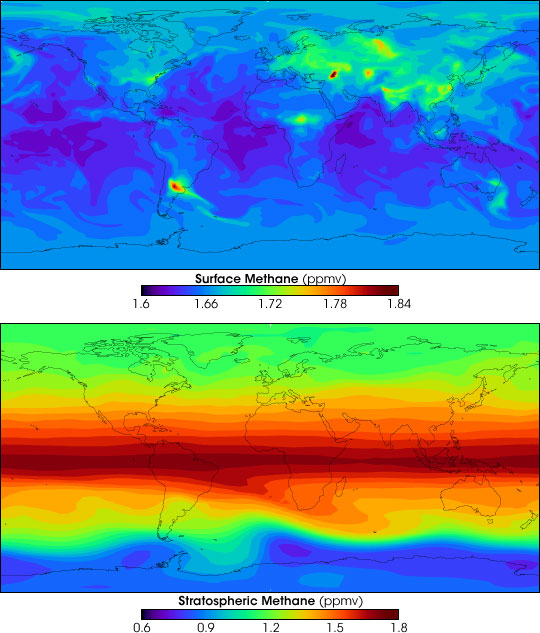
\includegraphics[width=8cm]{fig/AtmosphericMethane.png}
    \caption{Simulaciones mostrando la concentración de metano cerca del suelo y metano estratosférico \cite{hu2018global}.}
    \label{fig:atmosphericMethane}
\end{figure}

\section{Planificación del proyecto}

En la siguiente sección se muestran los avances orientados a la organización y conceptualización del proyecto.

\subsection{Arquitectura preliminar del módulo}

El diagrama en bloques que se observa en la Fig.\ref{fig:payload} indica de manera preliminar todos los elemento a tener en cuenta para la realización del módulo para mapeo de gases contaminantes en la atmósfera.



\begin{figure}[htb!]
    \centering
    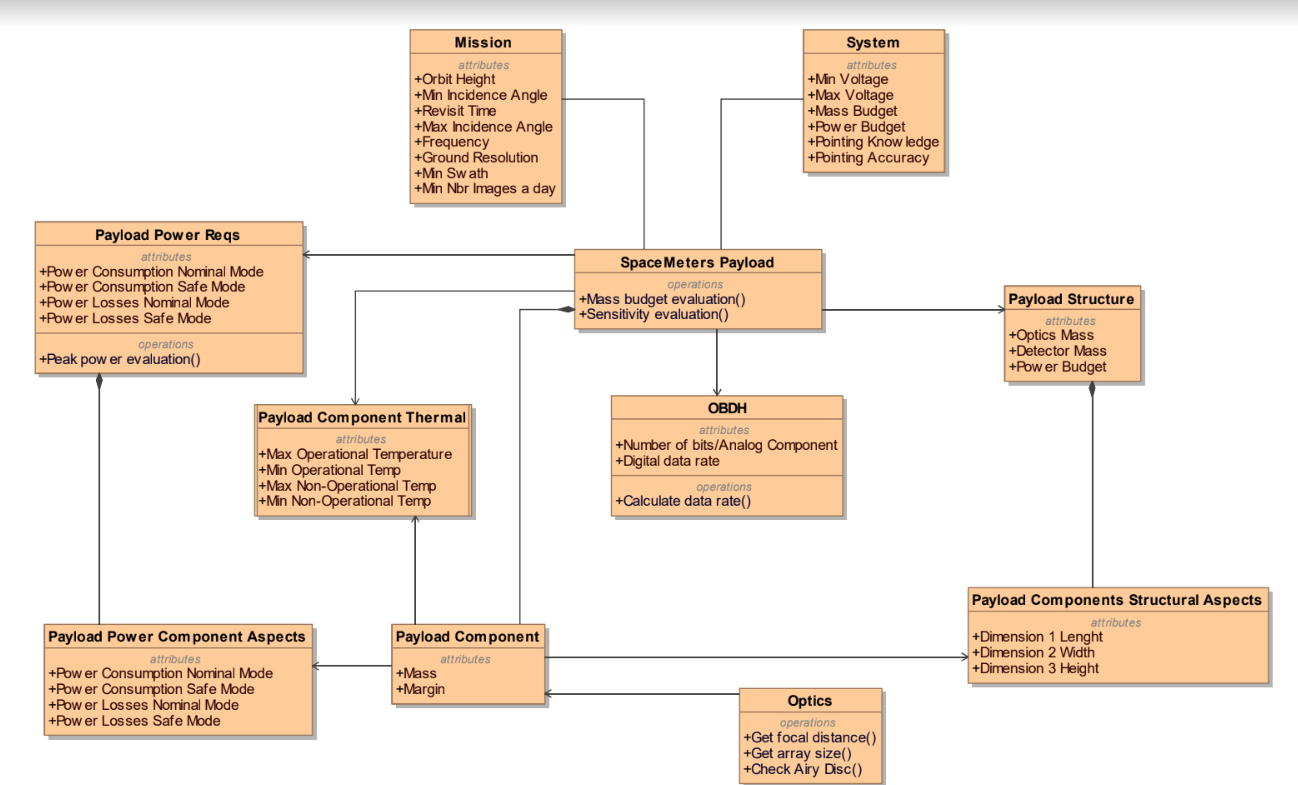
\includegraphics[width=15cm]{fig/payload.png}
    \caption{Diagrama en bloque de la arquitectura del módulo}
    \label{fig:payload}
\end{figure}

\subsection{Análisis de riesgos}

Este análisis resulta de suma importancia a lo largo de todo el proyecto, ya que permite anticiparse a posibles fallas en el momento de diseño, permite ver en qué elementos del proyecto prestar mayor atención y, finalizada cada etapa, permite identificar las lecciones aprendidas.
Para llevar a cabo esto, realizamos un análisis de las posibles problemáticas que se podrían generar durante la realización del proyecto y le asignamos una acción y un responsable para poder resolverla. El modo de cuantificar cada una de las tareas fue asignado un valor en función de la probabilidad de ocurrencia y la severidad de impacto, dando como resultado tres escalas representadas con tres colores diferentes:
\begin{itemize}
    \item Verde: Impacto bajo
    \item Amarillo: Impacto medio
    \item Rojo: Impacto alto
\end{itemize}

\begin{figure}[htb!]
    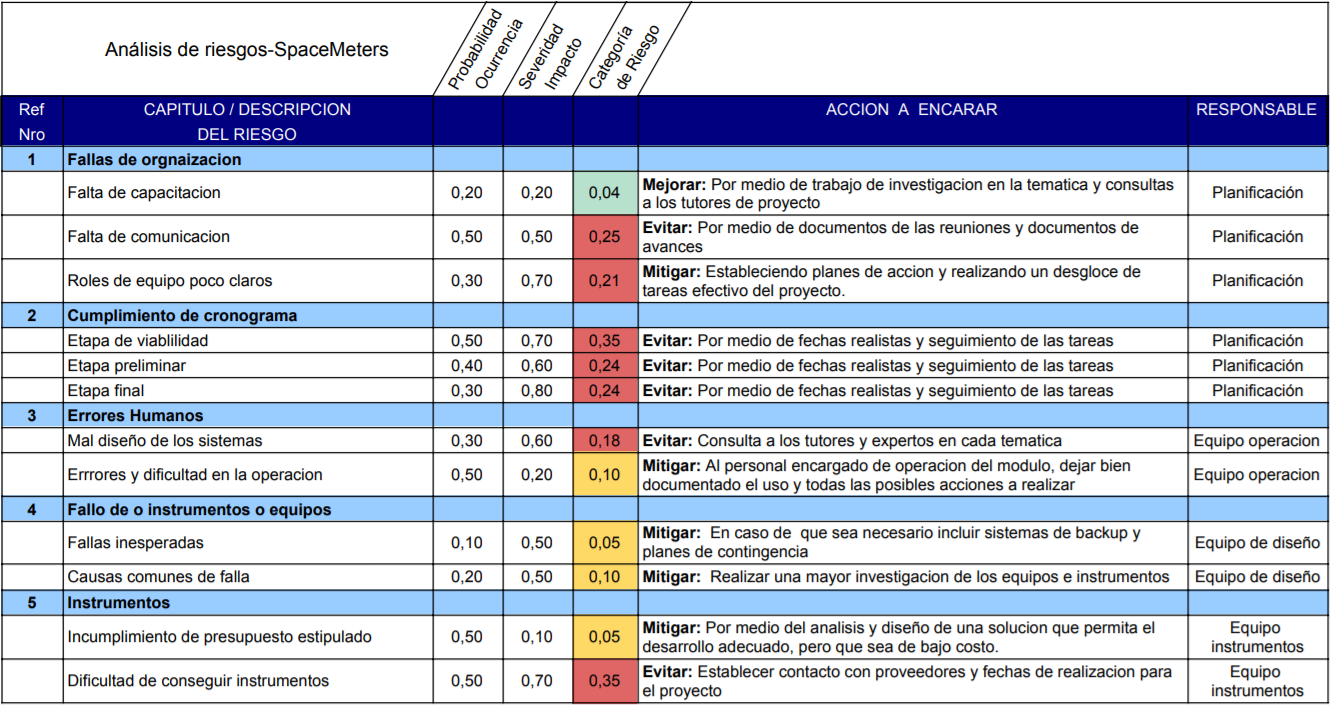
\includegraphics[width=18cm]{fig/riesgos.png}
    \caption{Análisis de riesgos de proyecto}
    \label{fig:my_label}
\end{figure}

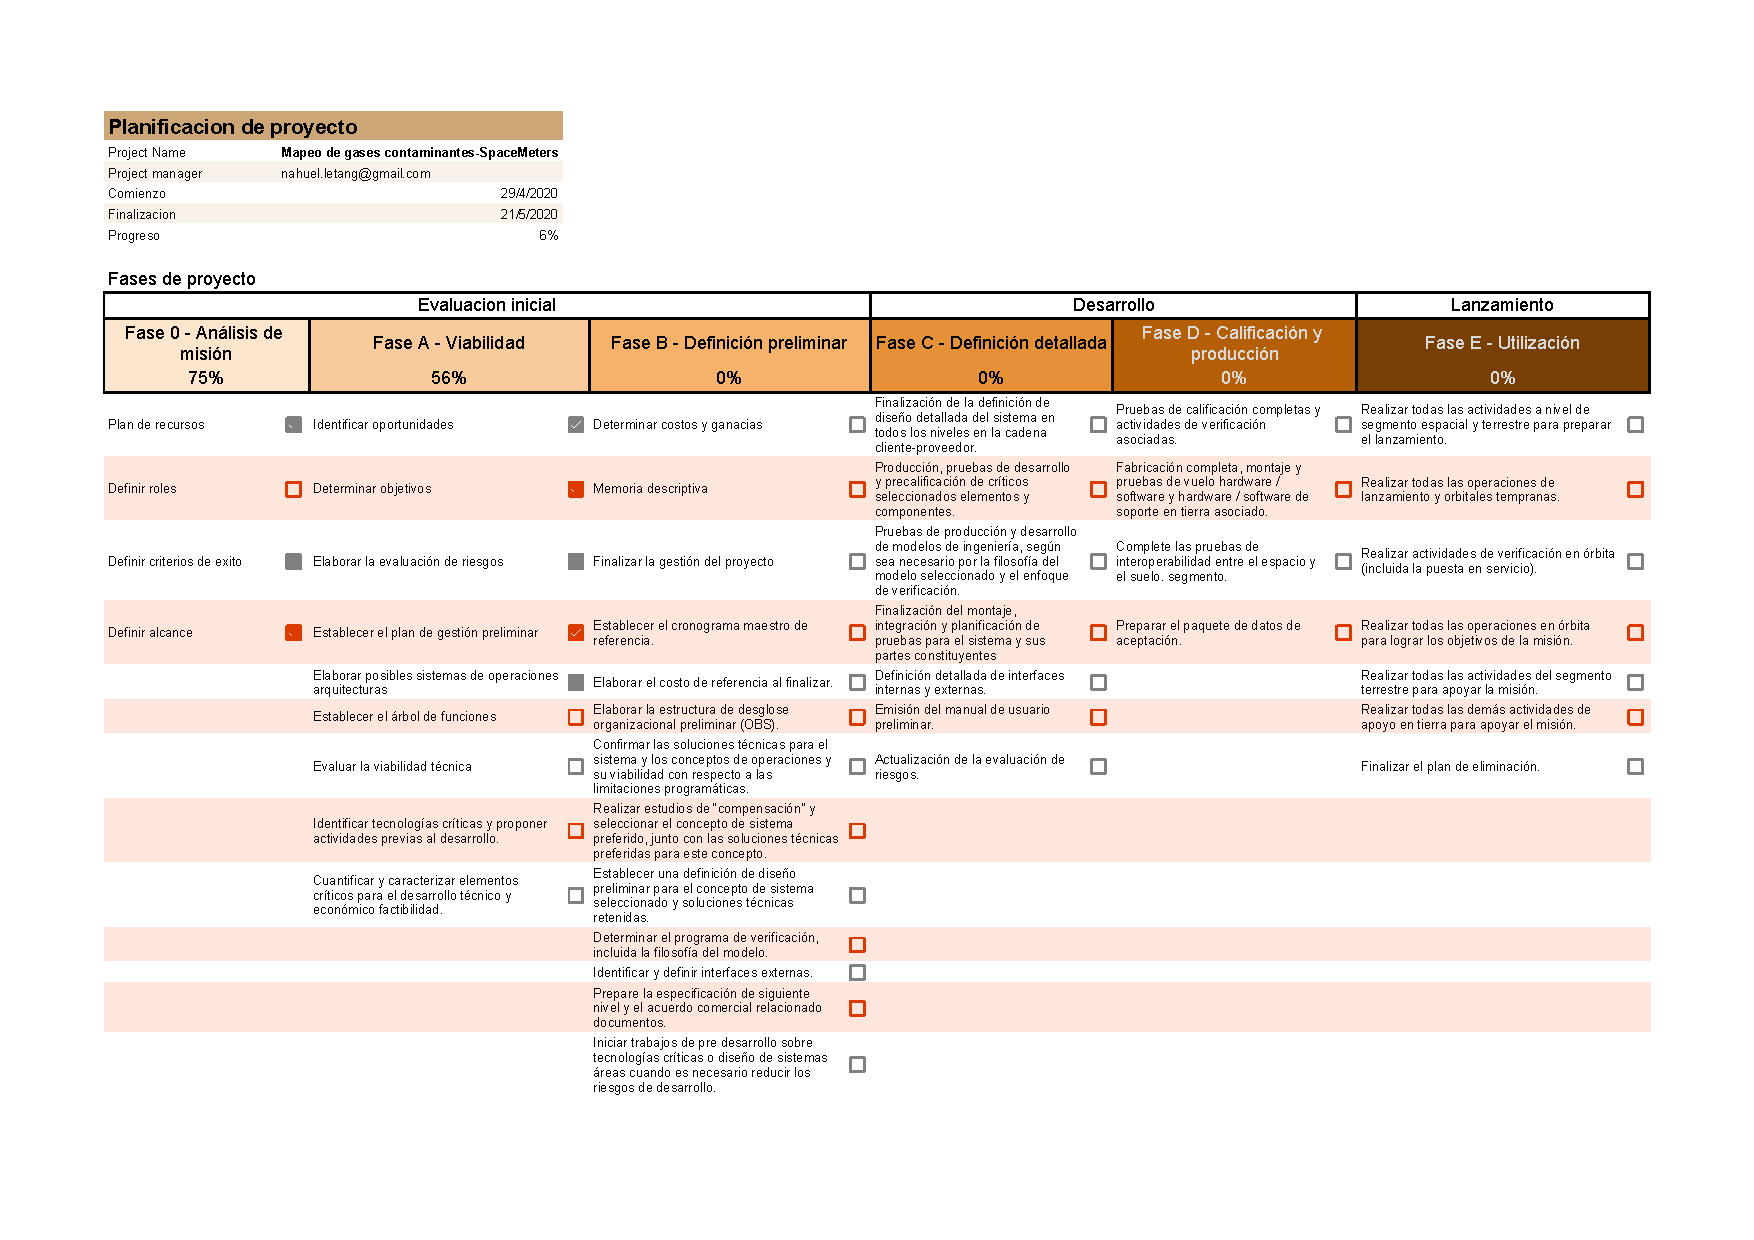
\includepdf[fitpaper, pages={1,2}]{pdf/planificacionProy}
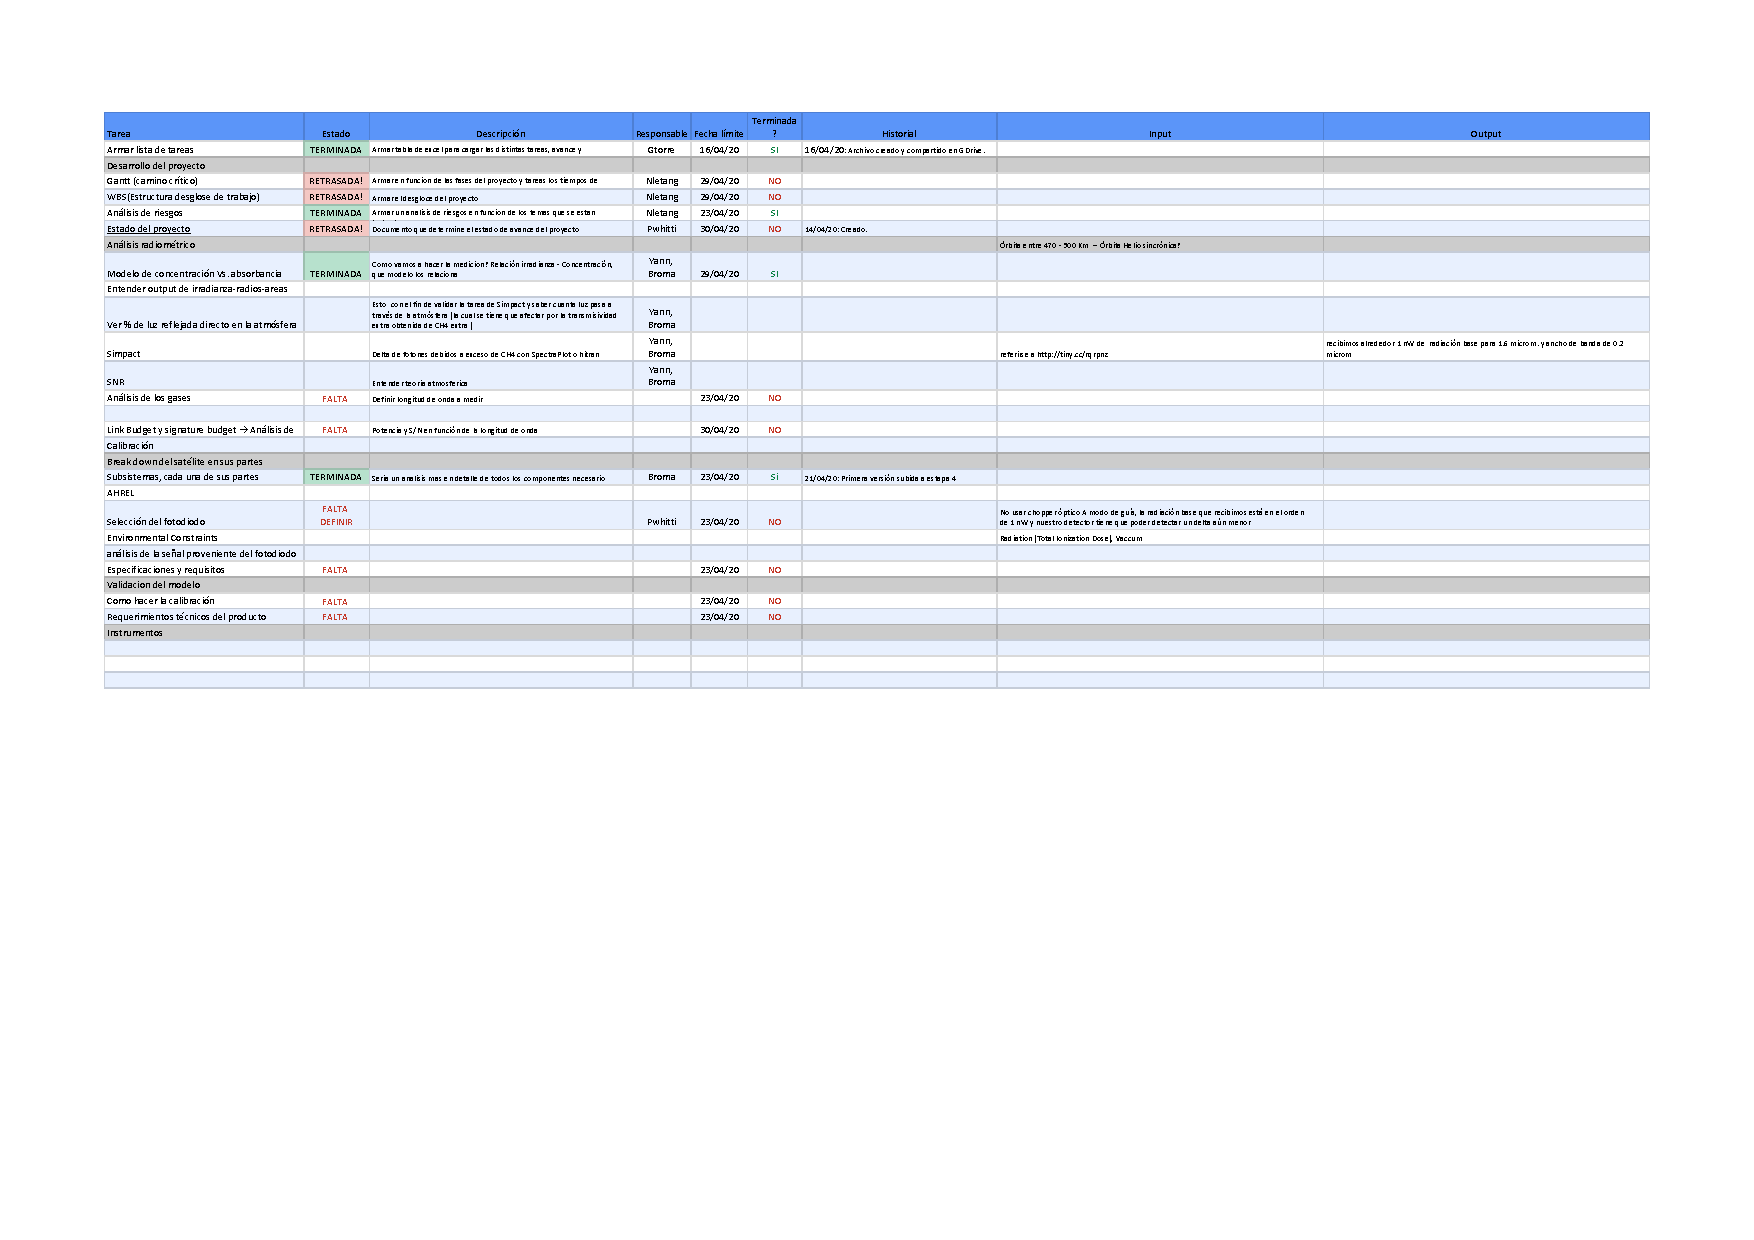
\includepdf[fitpaper]{pdf/tareas}

\newpage
\section{Análisis de gases}

Uso de la librería \texttt{py6s} con Colab.
Para utilizar \texttt{py6s} desde el Colab la primera vez, hay que correr el script desde el principio para que se instalen todos los componentes y luego correr el código. La librería tiene perfiles atmosféricos precargados, por lo tanto le cargamos el modelo de la atmósfera según nuestro caso.
Con la siguiente función, especificamos las longitudes de onda, para un gas determinado:

\begin{lstlisting}
wavelengths, ch4 = SixSHelpers.Wavelengths.run_wavelengths(s, np.arange(1,4,0.01),
output_name='transmittance_ch4.total')
\end{lstlisting}

\subsection{Curvas de absorción del \metano}

A través de la librería mencionada anteriormente se realizó un análisis del espectro de gases en la atmósfera, en donde hicimos particular énfasis en la detección del metano y la influencia de los otros gases a diferentes longitudes de onda, realizado en el siguiente \href{https://drive.google.com/open?id=1dH4wrmwYlQlsIZE5aXH2mcc7xXUcFgpj}{código}.

Primero analizamos la transferencia del metano y vemos que presenta picos de absorción en 1.6, 2,4 y 3.3 µm como se muestra en la Figura 1, donde se puede observar que el valor de intensidad en el pico de absorción se incrementa a medida que aumenta el rango de longitud de onda.

\begin{figure}[htb!]
    \centering
    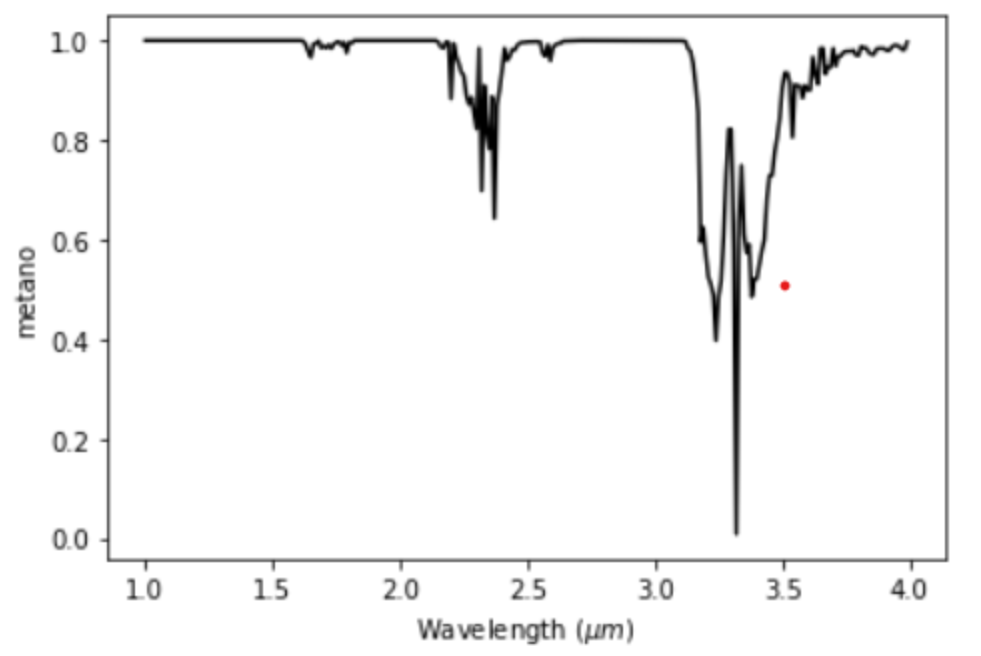
\includegraphics[width=10cm]{fig/absorbmetano.png}
    \caption{Absorción del metano Vs longitud de onda}
    \label{fig:absorbMetano}
\end{figure}


Luego nos enfocamos en medir únicamente los rangos de longitud de onda de interés, haciendo hincapié en los tres picos de absorción.
Analizando solamente el pico de los 1.6 µm como se muestra en la Figura 2, se puede observar que la influencia de los otros gases no es significante, pero tiene la característica que el pico de absorción es el más chico de los tres.

\begin{figure}[htb!]
    \centering
    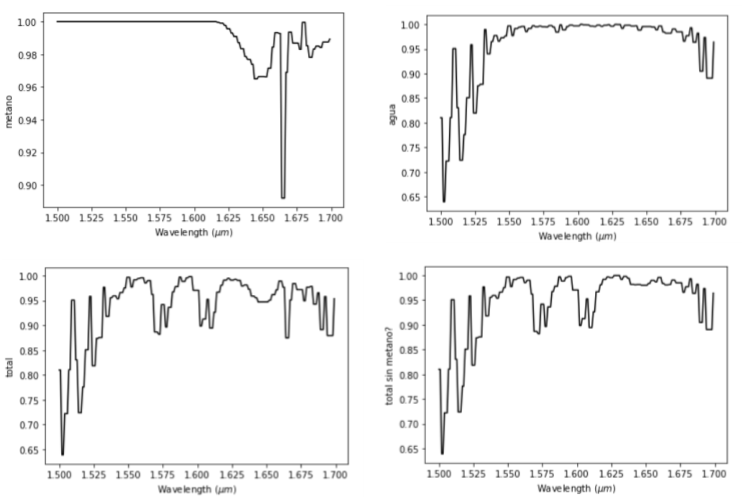
\includegraphics[width=15cm]{fig/analisis16.png}
    \caption{Análisis a 1.6 µm}
    \label{fig:analisis16}
\end{figure}


El segundo caso que analizamos fue el del rango de los 2.4 µm. Como se muestra en la Figura 3, se puede observar que el pico de absorción es mayor que el caso anterior pero la influencia del agua es significativa.

\begin{figure}[htb!]
    \centering
    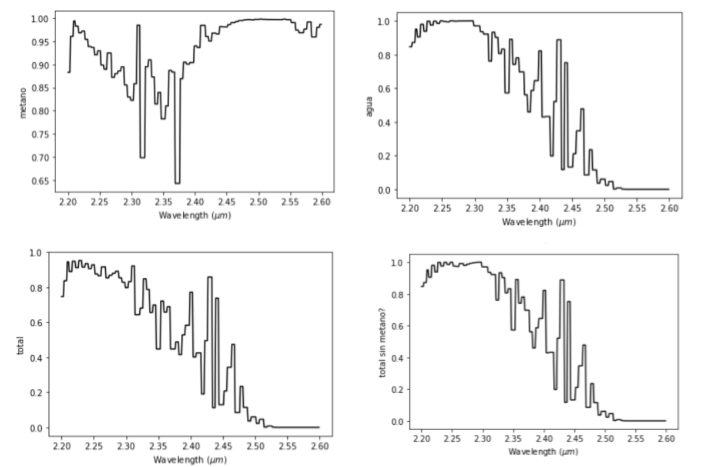
\includegraphics[width=15cm]{fig/analisis24.png}
    \caption{Análisis a 2.4 µm}
    \label{fig:analisis24}
\end{figure}


Por último, para el caso del rango de los 3.3 µm, como se muestra en la Figura 4 el pico de absorción es el mayor de todos para el metano, pero si analizamos la influencia del resto de los gases se puede ver que es muy significativa.
\begin{figure}[htb!]
    \centering
    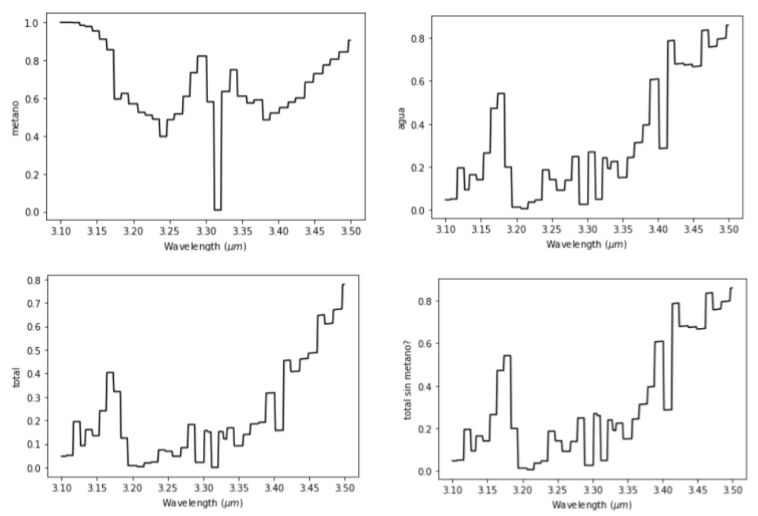
\includegraphics[width=15cm]{fig/analisis33.png}
    \caption{Análisis a 3.3 µm}
    \label{fig:analisis33}
\end{figure}

Como conclusión, podemos decir que de las tres longitudes de onda la que tiene menor influencia de los otros gases es la de 1.6 µm, pero también hay que analizar si el pico de absorción es lo suficientemente grande para poder ser detectado y, además, hay que considerar la influencia del piso de ruido que tengamos en la medición.

\subsection{Comparación con con mediciones de otros satélites}

El siguiente \href{https://www.atmos-chem-phys.net/16/14371/2016/acp-16-14371-2016.pdf}{documento} hace un análisis del modelo teórico que emplean en distintas misiones para medir metano. Resulta interesante la Tabla 1 del mismo, donde se especifica la resolución y el rango de longitud de onda empleado para medir metano. Esto nos resulta de mucha utilidad para complementar con el análisis del punto anterior, para definir qué rango de longitud de onda nos conviene medir.

 Por lo tanto, decidimos que un punto interesante para seguir trabajando es la misión correspondiente al \href{https://www.spiedigitallibrary.org/conference-proceedings-of-spie/10563/105634O/Fourier-transform-spectrometer-on-GOSAT-and-GOSAT-2/10.1117/12.2304062.full?SSO=1}{GOSAT} (enlace con información interesante sobre los datos constructivos de este satélite).
 
\subsection{Modelo teórico de cómo analizar y medir \metano}
Resulta de suma importancia entender la base teórica de lo que queremos medir para poder seguir avanzando con el análisis, para ello en el documento anterior hace una referencia breve a como lo realizaron en cada misión, en este documento se hace un mayor hincapié en la base teórica para medir metano en las diferentes misiones, considerando que las técnicas varían en función del rango de longitud de onda que se desea medir.

\subsection{Simulación 6S}
Para obtener una primera aproximación de la influencia de la concentración de metano sobre la radiancia se simuló el siguiente caso:
\begin{itemize}
    \item Diurno, 11hs
    \item Vegetación verde. Superficie Lambertiana homogénea
    \item Clima tropical
    \item Altitud de fin de atmósfera 100km
    \item Rango de longitud de onda estudiado $\lambda \in \{ 1.62, \, 1.70\}$ \micro m
\end{itemize}

Se varió la concentración de metano en la atmósfera entre 0 y 3 ppm en pasos de 0.5 ppm y se obtuvo la superficie mostrada en la figura \ref{fig:ch4IrrVsPpm}.


\begin{figure}[htb!]
\centering
\pgfplotsset{colormap/jet}
	\begin{tikzpicture}	
		\begin{axis}[view={30}{40}, width=0.8\textwidth,y dir=reverse,
		title={Radiancia de píxel a 100km de altura},xlabel={Longitud de onda [\micro m]},
		ylabel={Concentración de \metano [ppm]}, zlabel={\pixrad~  [\pixradunits]}]
		\addplot3 [surf, mesh/rows=7, shader=faceted interp]
		table[x=wl, y=ch, z=ir, col sep=comma] {plots/ch4ppmSurf-M7.csv};
		\addplot3 [mesh, black, mesh/rows=7, shader=faceted interp]		table[x=wl, y=ch, z=ir, col sep=comma] {plots/ch4ppmSurf-M7.csv};
		\end{axis}
	\end{tikzpicture}
	\caption{Grafico  de radiancia de píxel en función de longitud de onda y concentración de \metano.}
	\label{fig:ch4IrrVsPpm}
\end{figure}

\subsection{Simulaci\'on Spectraplot}
Se obtuvieron datos de absorción de luz para una columna de \metano~ utilizando la herramienta Spectraplot \cite{goldenstein2017spectraplot}. Se quiso obtener la absorbancia del \metano~ como lo vé 6S. Las variables de entrada fueron

\begin{itemize}
    \item Longitud de medio $L=100$km. En concordancia con la longitud para la cual integra 6S.
    \item Concentración constante de \metano~ 3 ppm
    \item Mismo rango de longitud de onda: $\lambda \in \{1.62,\,1.70\}$
    \item Temperatura constante 253K.
    \item Presión constante de 0.35 atm. Es un promedio efectivo de presión ya que la presión no varía linealmente entre 0 y 100 km. \footnote{Cabe destacar que la hipótesis de continuidad deja de ser valida a partir de los 60km y por ende no tiene sentido de hablar de una presión a partir de esta altura. Se podría tomar esto en cuenta para futuros analisis.}
\end{itemize}

con estos datos se obtuvo la transmitancia $T = \frac{I}{I_0}$ (figura \ref{fig:transmitancia100km3ppm}).

\begin{figure}[htb!]
    \centering
	\begin{tikzpicture}
	\begin{axis}[width=0.6\textwidth, title={Transmitancia de una columna de \metano~ de 100km, 3ppm a 0.35atm},xlabel={Longitud de onda [\micro m]},
	ylabel={Transmitancia $\frac{I}{I_0}$}, xmax=1.7,xmin=1.62]
	\addplot[blue] [thick,grid=both]
	table[x=x, y=y, col sep=comma] {plots/trans-3ppm-100km.csv};
	\end{axis}
	\end{tikzpicture}
    \caption{Gráfico obtenido combinando varios resultados del Spectraplot.}
    \label{fig:transmitancia100km3ppm}
\end{figure}


\subsection{Comparaci\'on de resultados entre 6S y Spectraplot}
Se busca comparar los resultados de superponer los efectos de la columna de \metano~ del Spectraplot con los del 6S. Para tal efecto se multiplica la intensidad obtenida del 6S para 0 ppm de \metano~ por la transmitancia obtenida del Spectraplot. Esto resultó en lo que llamaremos una radiancia de píxel modificada. Este perfil de radiancia de píxel fue comparado con la radiancia de píxel obtenida del 6S para 3 ppm haciendo una integración sobre el rango de longitud de onda para obtener la radiancia $\radiance$
\begin{equation}
    \radiance = \int_{\lambda_1}^{\lambda_2} \left.\pixrad(\lambda)\right|_{\text{3ppm}}  \diff \lambda \qquad [\radianceunits] 
\end{equation}
\begin{equation}
    \radiance = \int_{\lambda_1}^{\lambda_2} \left.\pixrad(\lambda)\right|_{\text{0ppm}} \cdot T(\lambda) \diff \lambda \qquad [\radianceunits] \quad \text{Radiancia modificada}
\end{equation}

Los valores obtenidos de radiancia nos dicen el área bajo las curvas de radiancia de pixel. Estos valores son una medida de la potencia que va recibir el sensor. Las radiancias de pixel se muestran en la figura \ref{fig:irradianzasComparativo} y las radiancias integrada se muestran en la tabla \ref{tab:radianciasYModificada}. Se puede observar que la disminución/atenuación de radiancia es del mismo orden de magnitud y difiere poco. La rutina de python que efectuó el cálculo se puede encontrar en \href{https://github.com/spacemeters/radiometry/blob/master/etapa4/validation.py}{github.com/spacemeters/radiometry}.

\begin{table}[htb!]
    \centering
    \begin{tabular}{lcc}
        \textbf{Caso} & \radiance [\radianceunits] & Atenuación [\%] \\ \hline
          \pixrad~ para 0ppm & 1.0858 & Referencia \\
          \pixrad~ para 3ppm & 1.0480 &  3.5\% \\
         \pixrad~ modificada & 1.0339 & 4.8\%
    \end{tabular}
    \caption{Radiancias para dos simulaciones de 6S y una simulación de 6S afectada por la transmitancia obtenida de Spectraplot.}
    \label{tab:radianciasYModificada}
\end{table}




\begin{figure}[htb!]
    \centering
	\begin{tikzpicture}
		\begin{axis}[width=0.8\textwidth, title={Radiancia de pixel vs. longitud de onda}, ylabel={$\pixrad$ [\pixradunits]}, xlabel={Longitud de onda [\micro m]}, xmax=1.7,xmin=1.62]
		\addplot[orange] [grid=both]
		table[x=wl, y=IR, col sep=comma] {plots/modIR-3ppm-100km.csv};
		\addplot[blue,dotted] [ultra thick,grid=both]
		table[x=x, y=y, col sep=comma] {plots/IR0ppm.csv};
		\addplot[red] [thick,grid=both]
		table[x=x, y=y, col sep=comma] {plots/IR3ppm.csv};
		\legend{$\pixrad$ modificada,0ppm,3ppm}
		\end{axis}
	\end{tikzpicture}
    \caption{Resultados de simulación 6S para 0ppm/3ppm y una superposición del caso 0 ppm de 6S con los datos del Spectraplot ($\pixrad$ modificada).}
    \label{fig:irradianzasComparativo}
\end{figure}

	



\subsection{Cálculo de señal recibida}

Una vez obtenida la radiancia de píxel \pixrad~, se calcula la intensidad que llega al sensor según la altura del satélite $h_\LEO$ y el tamaño de píxel $A_\px$, el cual es el área observado sobre la tierra. 

\begin{equation}
    I_\sensor(\lambda) =  \frac{A_\px}{(R_\earth+h_\LEO)^2} \cdot  \pixrad(\lambda) \qquad [\text{W m}^{-2}\, \micro\text{m}^{-1} ] 
\end{equation}

El sensor convierte fotones a electrones. Nos interesa obtener el flujo de fotones sobre la superficie y según la longitud de onda. La energía de un fotón es dada por $E_f = \frac{hc}{\lambda}$ 

\begin{equation}
    \Phi_\sensor(\lambda) = \frac{I}{E_f} = \frac{I_\sensor(\lambda) \cdot \lambda }{hc} \qquad [\text{fotones m}^{-2}\, \micro \text{m}^{-1}] 
\end{equation}

Luego, multiplicando el valor $\Phi_\sensor$ por el área del sensor se obtiene la cantidad de fotones que inciden sobre el sensor. Para obtener la cantidad de electrones generados en corriente se integra la expresión obtenida multiplicada por la \gls{quantumeff} $Q$ del sensor, la cual también depende de la longitud de onda del fotón incidente.

\begin{equation}
    n_e = \int_{\lambda_1}^{\lambda_2} A_\sensor \cdot\Phi_\sensor(\lambda) Q(\lambda) \diff \lambda  \qquad [\text{electrones  s}^{-1}]
\end{equation}

La señal obtenida va ser la corriente, dada por
\[
i_\sensor = n_e\cdot q_e = n_e \cdot 1.602176634\times10^{-19} \qquad [\text{Amperes}]
\]
siendo $q_e$ la carga del electrón.
Es necesario aún efectuar el análisis de \textit{signal to noise ratio} (S/N) partiendo del sensor elegido. A continuación se detalla un ejemplo del cálculo que se debería hacer suponiendo algunos valores

\begin{itemize}
    \item Área de sensor $50$mm$^2$
    \item Área de pixel observado de 100km$^2$ (área de Manhattan)
    \item Variación de 1\% de la potencia recibida, que podría corresponder a una variación de 1ppm de \metano~ en la atmósfera según la tabla \ref{tab:radianciasYModificada}
    \item Quantum efficiency igual a 50\% constante
\end{itemize}

\[
\Delta i_\sensor = \Delta n_e \cdot q_e = \frac{A_\sensor A_\px \cdot q_e}{h c (R_\earth + h_\LEO)^2 } \cdot \int_{1,62}^{1.70} \lambda \cdot\Delta \pixrad(\lambda) Q(\lambda) \diff \lambda = 2.4\times 10^{-18} \text{A}
\]
La pregunta es contundente ¿como medimos esta corriente?

Formas de aumentar $\Delta i_\sensor$:
\begin{itemize}
    \item Acercarse lo más posible al rango de longitudes de onda donde el CH4 tiene más influencia (entre 1.665 y 1.6675)
    \item Aumentar $A_\px$, tener en cuenta la distancia focal.
    \item Aumentar $A_\sensor$, limitado por espacio disponible y lentes.
    \item Cambiar el modo de vibración observado a alguno que presente mayor absorbancia.
\end{itemize}{}
\section{Construcción del monocromador}
En función de lo dicho anteriormente y basados en el diseño de una misión que se realizó anteriormente hay que definir qué sistema vamos a usar y qué componentes son cruciales, cómo se desarrolló en el siguiente \href{https://drive.google.com/drive/u/1/folders/1x8ssW4P_UQonP1F5NF6wIi2mThU0y0k_}{documento}.

\subsection{Base teórica}
Un monocromador es un dispositivo óptico que sirve para medir la composición de la luz según su distribución de longitudes de onda (distribución espectral) ya sean electromagnéticas o no a partir de una fuente emisora que produzca una amplia gama de longitudes de onda.

\subsection{Análisis de componentes}
\begin{description}
    \item[Espejos] 	 \href{https://www.thorlabs.com/newgrouppage9.cfm?objectgroup_id=1161}{siguiente enlace} son espejos comerciales a modo de ejemplo, sin embargo excedemos el rango de longitudes de onda de estos espejos en particular
    \item[Red de difracción] 
    \item[Rendijas] 
\end{description}

\subsection{Posibles diseños}
Una idea es agregarle un espejo móvil o un diseño con un chopper mas complejo que deje pasar dos caminos de luz alternativamente. Porque si necesitamos medir más de una longitud de onda, y comprar analizadores que miden un mayor espectro, esta solución permite barrer en longitudes de onda empleando un solo sensor y de forma mucho más económica.

Considerar de construir con más de un sensor, pero para ello hay que tener una base teórica más amplia.

\subsection{Planes de contingencia}
Se puede considerar la idea de tener un sensor de backup, en caso de alguna falla.

\section{Fotodiodo}
Lead Sulfide (PbS) y Lead Selenide (PbSe) se usan mucho en la detección infrarroja desde 1000 nm hasta 4800 nm. 
Justo el fotodiodo que elegimos (FDPS3X3) a diferencia de los fotodiodos estándares que producen corriente cuando reciben luz, reduce la resistencia eléctrica del material fotoconductivo al iluminarse. El manual indica que la luz incidente disminuye la resistencia del detector, provocando un cambio en el voltaje medido y en la fotosensibilidad. Más detalle \href{https://www.thorlabs.com/drawings/53832b2035a4b665-C7A783DC-C708-1572-7544F10825D99274/FDPS3X3-Manual.pdf}{aquí}.

Por otro lado, según el mismo manual, los fotodiodos se tienen que usar con una señal pulsante para así obtener una salida AC. Recomiendan usar un optical chopper (es un disco con agujeros que al girar hace intermitente la señal) tal como este para tener una Constant Wave light:

\begin{figure}[htb!]
    \centering
    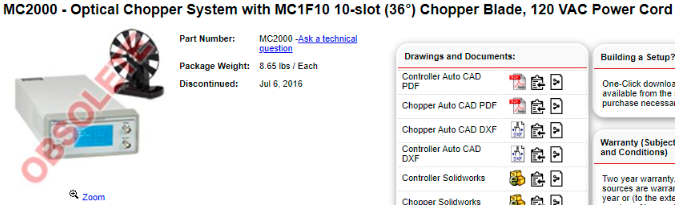
\includegraphics[height=4cm]{fig/wavechopper.png}
    \caption{\textbf{Notar:} la imagen dice obsolete.}
    \label{fig:wavchopper}
\end{figure}

Se recomienda un input AC debido a las características que tiene el fotoconductor con el ruido. Sino el ruido (en DC) presente con el bias aplicado serìa muy grande a altos niveles de bias, limitando la practicidad del detector.

Por esa razón detectores IR se utilizan con AC para limitar el ruido.
Generalmente los PbS y PbSe detectors tienen un espectro de ruido de 1/f, es decir que disminuye el ruido a medida que aumenta la chopping frequency.

\begin{figure}[htb!]
    \centering
    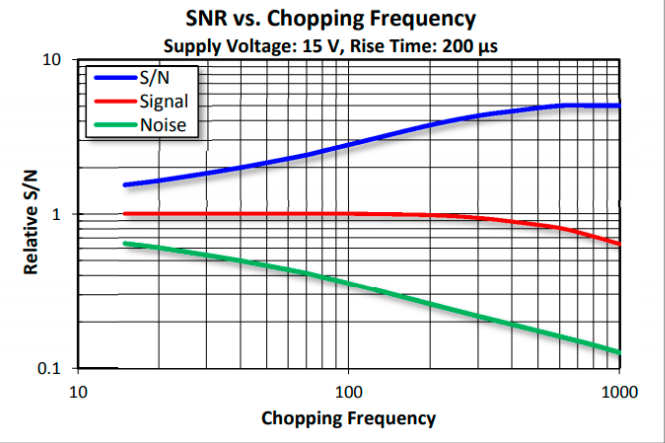
\includegraphics[height=7cm]{fig/snrchopfreq.png}
    \caption{Visualización de cambio en la relación S/N según la frecuencia de chopping.}
    \label{fig:snrChopFreq}
\end{figure}

\subsection{Circuito típico de amplificación}
Se necesita un pre-amplificador para mantener la estabilidad y proveer gran ganancia de la señal. Más info \href{https://www.thorlabs.com/drawings/53832b2035a4b665-C7A783DC-C708-1572-7544F10825D99274/FDPS3X3-Manual.pdf}{aquí}.


\clearpage
\section{Anexos}

\addcontentsline{toc}{subsection}{\listfigurename}
\listoffigures
\addcontentsline{toc}{subsection}{\refname}

\subsection{\href{https://drive.google.com/open?id=1XFQf_anSSaL9RTy9PBaxXfIFHyrzE6CN}{Informe I-SpaceMeters}}
\subsection{\href{https://drive.google.com/open?id=1-w1e1fudWwtTKKnJxD-XJ_QvBDY1P5ty}{Informe II-SpaceMeters}}

\bibliography{biblio}
%\addcontentsline{toc}{subsection}{\lstlistlistingname}

\end{document}